\documentclass[12pt,a4paper]{article}
\usepackage[utf8]{inputenc}
\usepackage[T1]{fontenc}
\usepackage[spanish]{babel}

\usepackage[margin=2.5cm]{geometry}
\usepackage{microtype}
\usepackage{graphicx}
\usepackage{amsmath,amssymb}
\usepackage{bm}
\usepackage{csquotes}
\usepackage{xcolor}
\usepackage{booktabs}
\usepackage{enumitem}
\usepackage{hyperref}
\usepackage{authblk}
\usepackage{fancyhdr}
\usepackage{lastpage}
\usepackage[spanish]{cleveref}
\usepackage{derivative}
\usepackage{siunitx}
\usepackage{float}

\hypersetup{
  colorlinks=true,
  linkcolor=black,
  urlcolor=blue,
  pdftitle={Report Finite Differences},
  pdfauthor={Avila, Huertas, Rodríguez, Acuña},
  pdfsubject={Finite Differences},
  pdfkeywords={Finite Differences}
}
\urlstyle{same}

\renewcommand{\vec}[1]{\boldsymbol{#1}}

\title{\textbf{Diferencias Finitas} \\ \small{Comparación entra Fortran, Python y Solución Analítica}}
\author{Julian Avila, Camilo Huertas, David Rodríguez, Juan Acuña}

\fancyhf{}
\lhead{\textit{Diferencias Finitas}}
\rhead{\textit{Avila, Huertas, Rodríguez, Acuña}}
\rfoot{Pagina \thepage\ de \pageref{LastPage}}
\pagestyle{fancy}

\begin{document}

\maketitle
\vspace{-1em}
\hrule
\vspace{1em}

Se solucionaron distintas Ecuaciones de Poisson con distintas
condiciones de frontera.
Se comparó el tiempo de ejecución para solucionar numéricamente por medio de
diferencias finitas usando Python y Fortran.
Se emplearon mallas de 100x100 con una tolerancia de $10^{-7}$.

\section*{Problema 1}%
\label{sec:Problema 1}

Ecuación diferencial:
\begin{equation}
  \nabla^2{V} = \left( x^2 + y^2 \right) e^{xy}
  \label{eq:1}
\end{equation}

Condiciones de frontera:
\begin{equation}
  V(x, y) =
  \begin{cases}
    V(0, y) = 1 & V(2, y) = e^{2y} \\
    V(x, 0) = 1 & V(x, 1) = e^{x}
  \end{cases}
\end{equation}

Solución Analítica:
\begin{equation}
  V = e^{xy}
\end{equation}

\subsection*{Resultados}%
\label{sub:Resultados-1}

\begin{table}[htbp!]
  \centering
  \begin{tabular}{@{}c|S[table-format=2.3]@{}}
    \toprule
    Lenguaje  & {Tiempo (s)} \\
    \midrule
    Fortran & 0.686 \\
    Python & 91.495 \\
    \bottomrule
  \end{tabular}
  \caption{Tiempo de ejecución \cref{eq:1}.}
\end{table}

\begin{figure}[H]
  \centering
  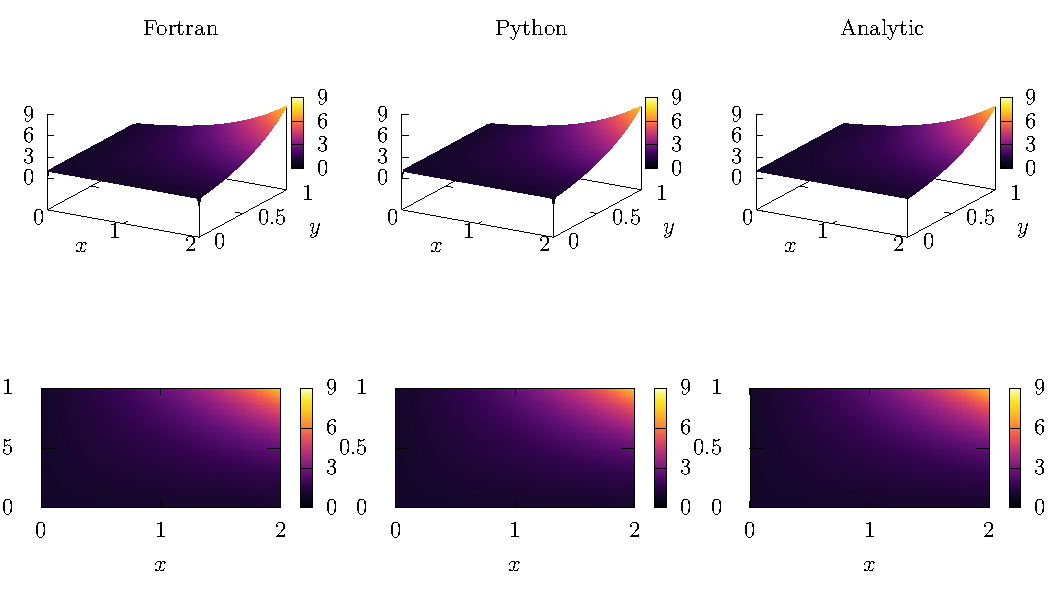
\includegraphics[width=\textwidth]{./comparison-01.pdf}
  \caption{Solución de la \cref{eq:1}}
  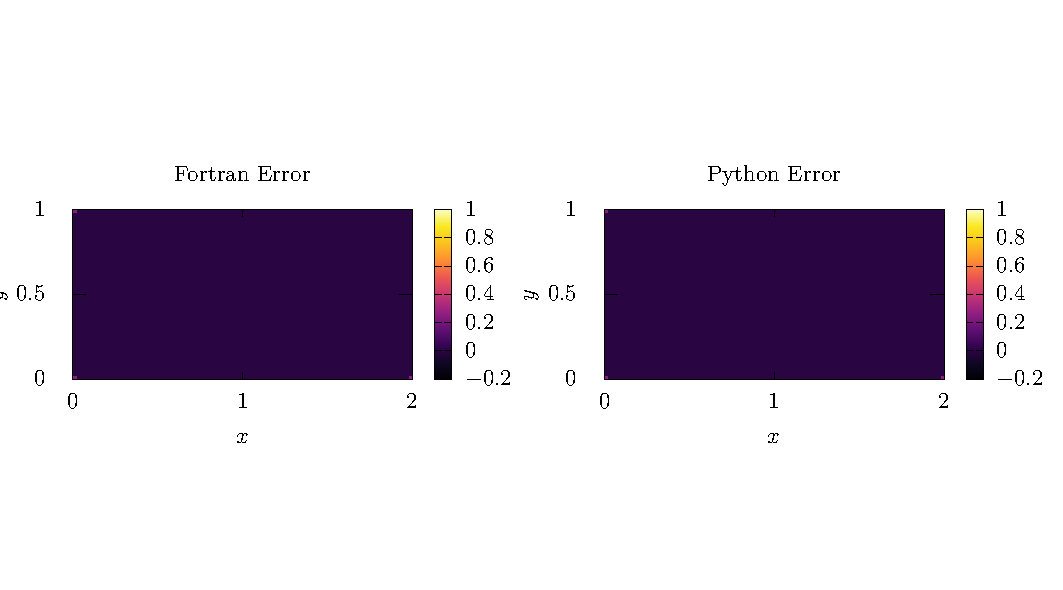
\includegraphics[width=\textwidth]{./error-01.pdf}
  \caption{Error de la solución}
\end{figure}

Se observa un error más elevado en las fronteras de la malla.

\newpage

\section*{Problema 2}%
\label{sec:Problema 2}

Ecuación diferencial:
\begin{equation}
  \nabla^2{V} = 0
  \label{eq:2}
\end{equation}

Condiciones de frontera:
\begin{equation}
  V(x, y) =
  \begin{cases}
    V(1, y) = \ln{\left(y^2 + 1\right)} & V(2, y) = \ln{\left(y^2 + 4\right)} \\
    V(x, 0) = 2 \ln{x} & V(x, 1) = \ln{\left(x^2 + 1\right)}
  \end{cases}
\end{equation}

Solución Analítica:
\begin{equation}
  V = \ln{\left(y^2 + x^2\right)}
\end{equation}

\subsection*{Resultados}%
\label{sub:Resultados-2}

\begin{table}[htbp!]
  \centering
  \begin{tabular}{@{}c|S[table-format=2.3]@{}}
    \toprule
    Lenguaje  & {Tiempo (s)} \\
    \midrule
    Fortran & 1.286 \\
    Python & 93.352 \\
    \bottomrule
  \end{tabular}
  \caption{Tiempo de ejecución \cref{eq:2}.}
\end{table}

\begin{figure}[H]
  \centering
  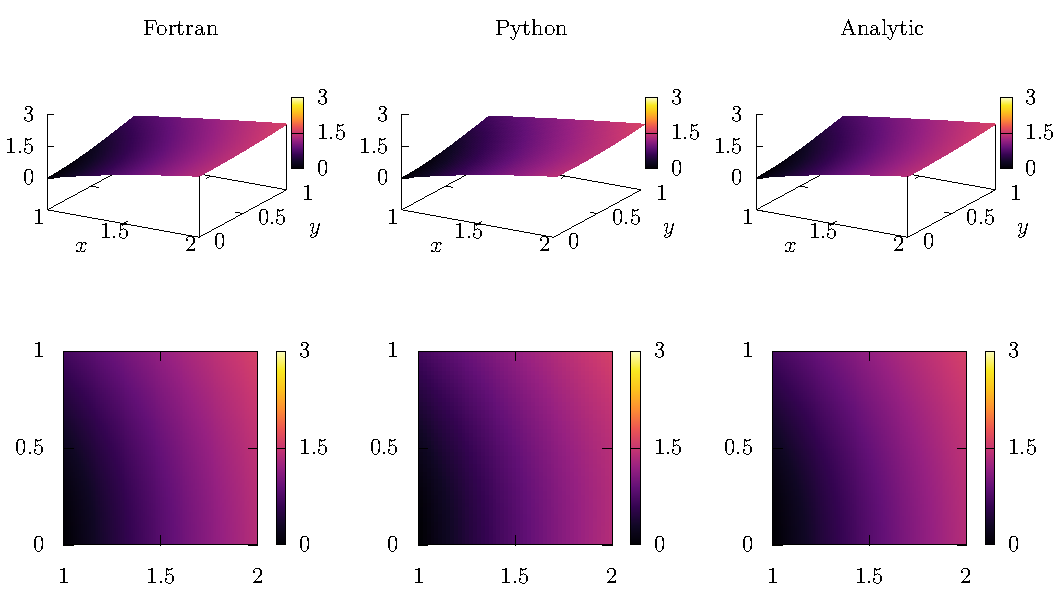
\includegraphics[width=\textwidth]{./comparison-02.pdf}
  \caption{Solución de la \cref{eq:2}}
  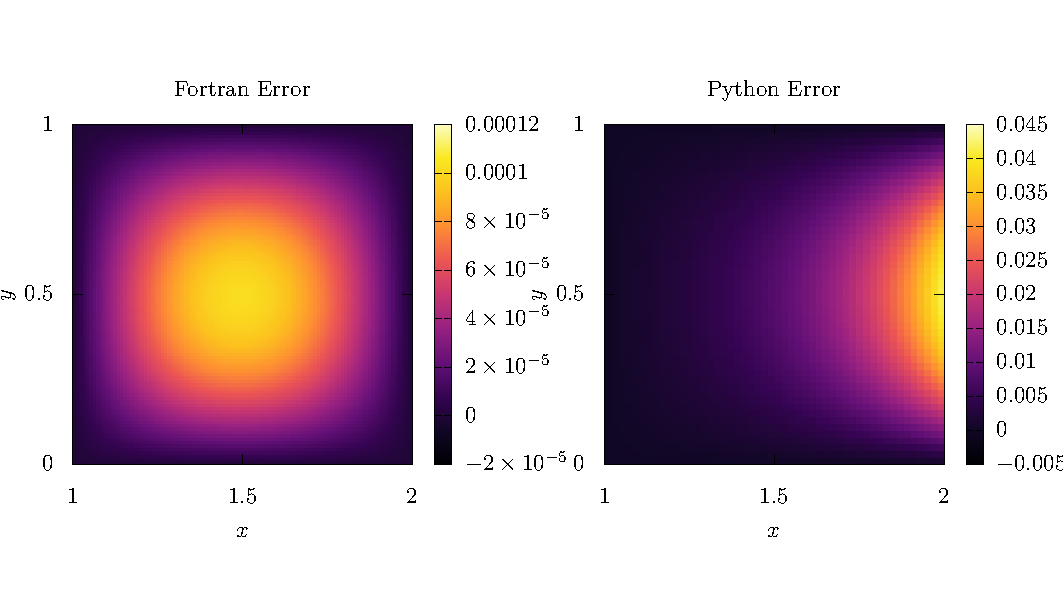
\includegraphics[width=\textwidth]{./error-02.pdf}
  \caption{Error de la solución}
\end{figure}

La solución obtenida con Fortran presenta un error menor en dos
órdenes de magnitud en comparación con la solución de Python.
En cuanto a la distribución espacial del error, la solución de
Fortran muestra los mayores errores en el centro de la malla,
los cuales disminuyen hacia los bordes, mientras que la de Python
presenta un error máximo en la frontera derecha, disminuyendo
progresivamente hacia la izquierda.

\newpage

\section*{Problema 3}%
\label{sec:Problema 3}

Ecuación diferencial:
\begin{equation}
  \nabla^2{V} = 4
  \label{eq:3}
\end{equation}

Condiciones de frontera:
\begin{equation}
  V(x, y) =
  \begin{cases}
    V(0, y) = y^2 & V(2, y) = (y - 2)^2 \\
    V(x, 0) = x^2 & V(x, 2) = (x - 2)^2
  \end{cases}
\end{equation}

Solución Analítica:
\begin{equation}
  V = (x - y)^2
\end{equation}

\subsection*{Resultados}%
\label{sub:Resultados-3}

\begin{table}[htbp!]
  \centering
  \begin{tabular}{@{}c|S[table-format=2.3]@{}}
    \toprule
    Lenguaje  & {Tiempo (s)} \\
    \midrule
    Fortran & 4.577 \\
    Python & 79.064 \\
    \bottomrule
  \end{tabular}
  \caption{Tiempo de ejecución \cref{eq:3}.}
\end{table}

\begin{figure}[H]
  \centering
  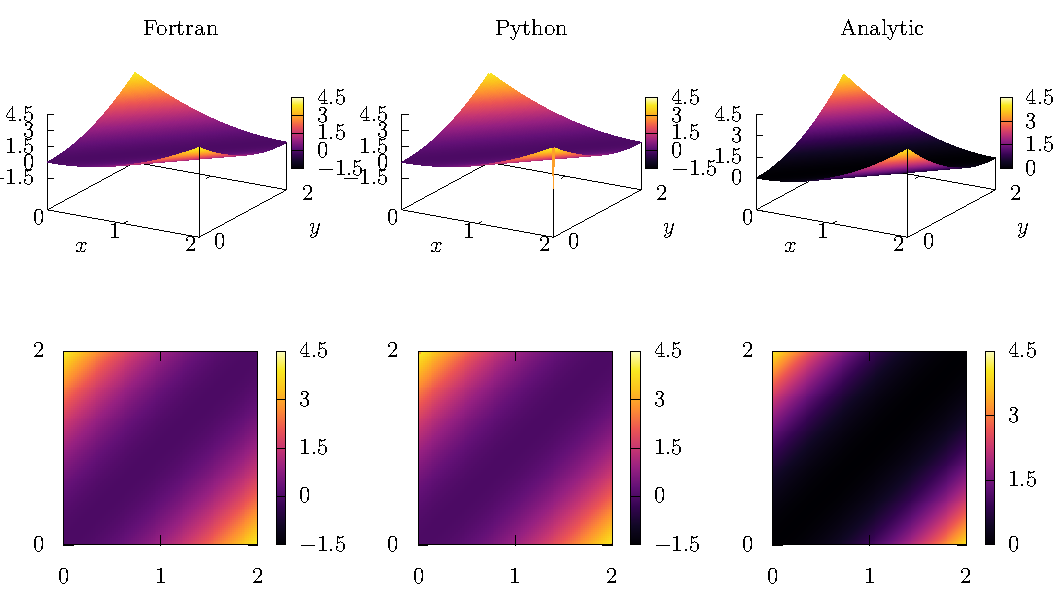
\includegraphics[width=\textwidth]{./comparison-03.pdf}
  \caption{Solución de la \cref{eq:3}}
  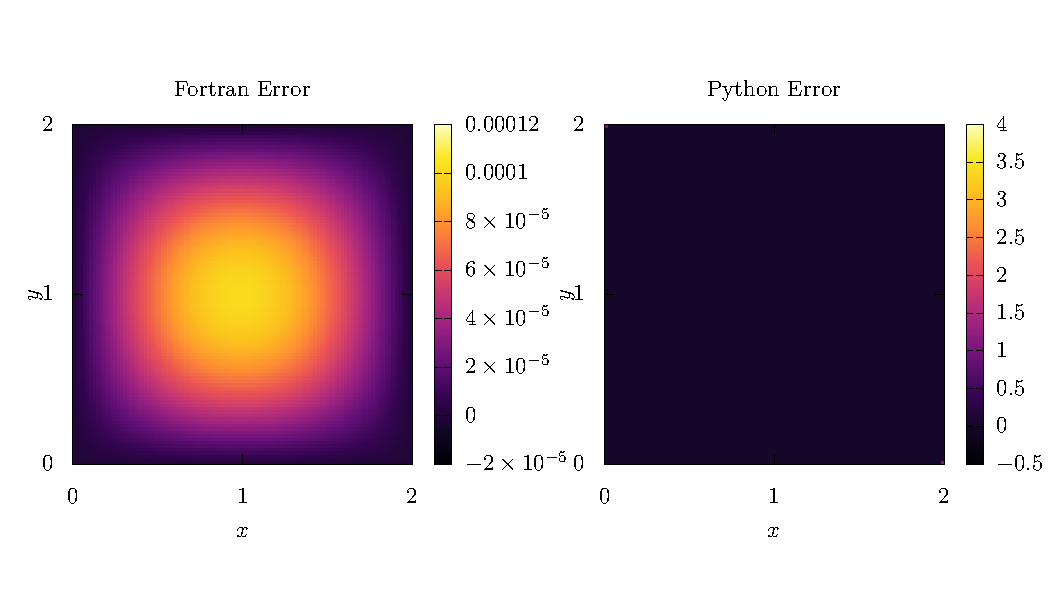
\includegraphics[width=\textwidth]{./error-03.pdf}
  \caption{Error de la solución}
\end{figure}

La solución de Fortran, nuevamente con un error menor, muestra una distribución
donde este disminuye radialmente a partir del centro de la malla.
En contraste, la solución de Python exhibe errores significativos en las
fronteras de la malla.

\newpage

\section*{Problema 4}%
\label{sec:Problema 4}

Ecuación diferencial:
\begin{equation}
  \nabla^2{V} = \frac{x}{y} + \frac{y}{x}
  \label{eq:4}
\end{equation}

Condiciones de frontera:
\begin{equation}
  V(x, y) =
  \begin{cases}
    V(1, y) = y \ln{y} & V(2, y) = 2y \ln{2y} \\
    V(x, 1) = x \ln{x} & V(x, 2) = 2x \ln{2x}
  \end{cases}
\end{equation}

Solución Analítica:
\begin{equation}
  V = xy \ln{xy}
\end{equation}

\subsection*{Resultados}%
\label{sub:Resultados-4}

\begin{table}[htbp!]
  \centering
  \begin{tabular}{@{}c|S[table-format=2.3]@{}}
    \toprule
    Lenguaje  & {Tiempo (s)} \\
    \midrule
    Fortran & 1.478 \\
    Python & 84.873 \\
    \bottomrule
  \end{tabular}
  \caption{Tiempo de ejecución \cref{eq:4}.}
\end{table}

\begin{figure}[H]
  \centering
  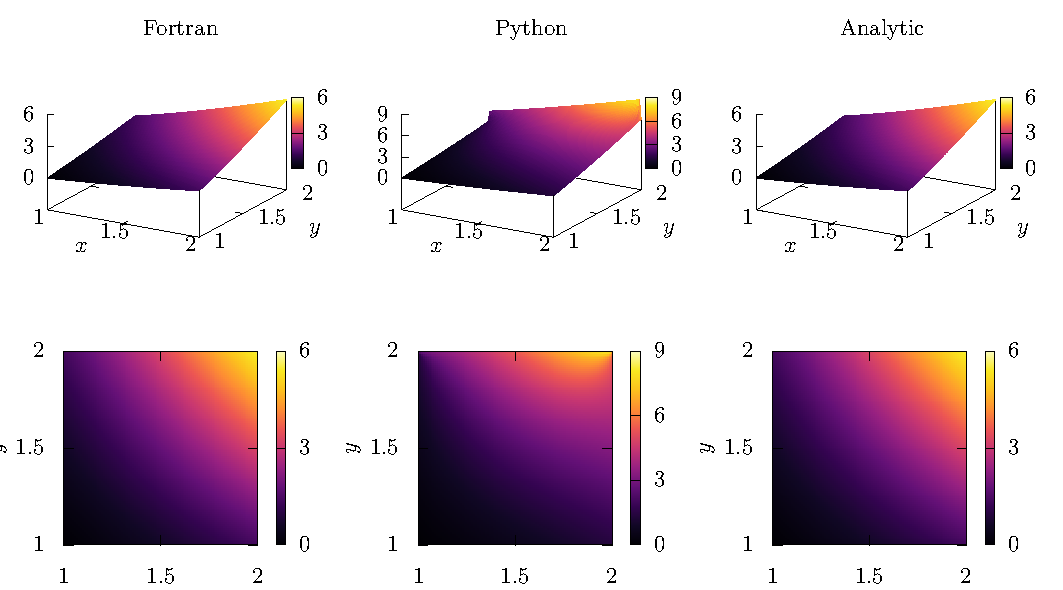
\includegraphics[width=\textwidth]{./comparison-04.pdf}
  \caption{Solución de la \cref{eq:4}}
  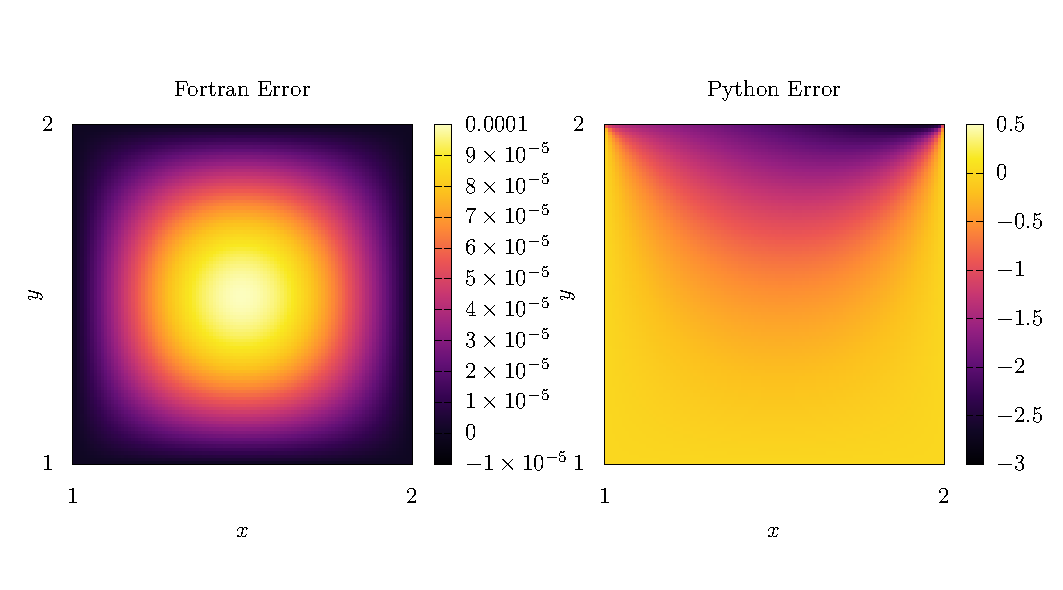
\includegraphics[width=\textwidth]{./error-04.pdf}
  \caption{Error de la solución}
\end{figure}

La solución de Fortran, nuevamente con un error menor, muestra una distribución
donde este disminuye radialmente a partir del centro de la malla.
En contraste, la solución de Python exhibe errores significativos en la
frontera superior, hay cuatro órdenes de magnitud de diferencia entre los errores
de los métodos.

\section{Tiempos}%
\label{sec:Tiempos}

Para la resolución de todas las Ecuaciones se emplearon las mismas condiciones
en ambos códigos. La ejecución en Fortran resultó sistemáticamente más rápida
que en Python, registrando diferencias que oscilaron entre 4 y 100 veces.

\end{document}
